\documentclass[tikz,border=10pt]{standalone}
\usepackage{tikz}
\usetikzlibrary{arrows.meta, positioning, fit, calc}

\begin{document}
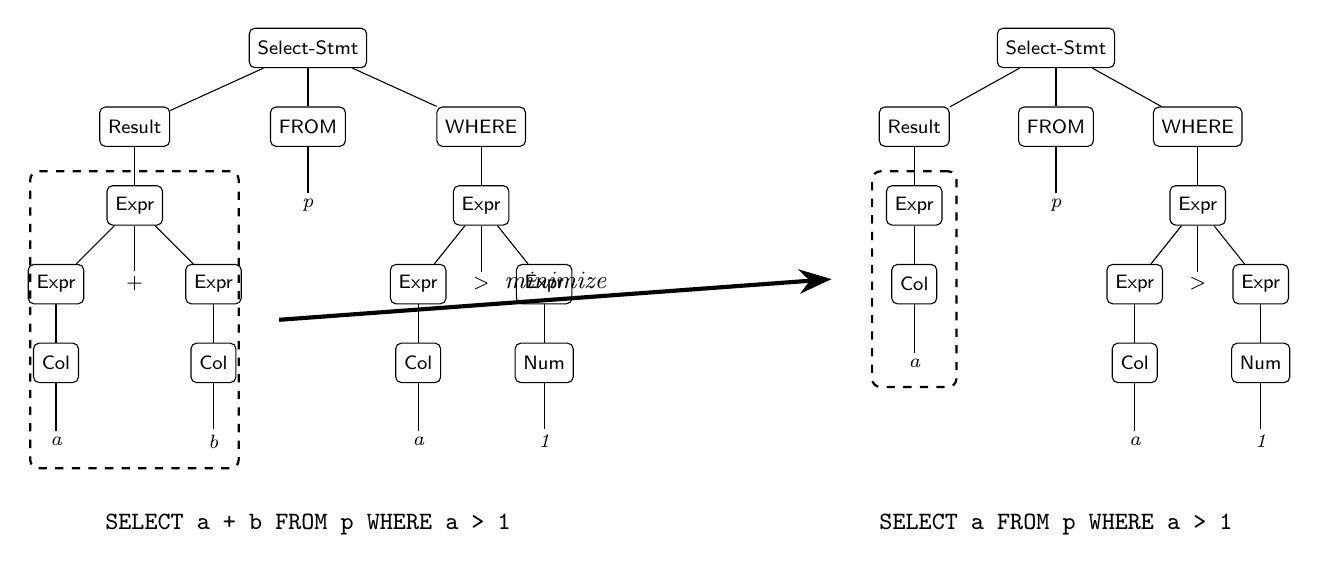
\begin{tikzpicture}[
    % Non-terminal: rounded rectangle with border
    nt/.style={
        rectangle, rounded corners=2pt, draw=black, thin,
        inner sep=3pt, minimum height=5mm,
        font=\scriptsize\sffamily
    },
    % Terminal: italic, no border
    t/.style={
        font=\scriptsize\itshape, inner sep=2pt
    },
    % Dashed highlight box
    hl/.style={
        draw=black, dashed, thick, rounded corners=3pt, inner sep=5pt
    },
    % Tree edge
    tedge/.style={thin, black},
    level distance=9mm,
    sibling distance=10mm,
]

% ============================================================
% LEFT TREE: SELECT a + b FROM p WHERE a > 1
% ============================================================

% Root
\node[nt] (L-sel) at (0, 0) {Select-Stmt};

% Level 1
\node[nt] (L-res)   at (-2.2, -1.0) {Result};
\node[nt] (L-from)  at ( 0.0, -1.0) {FROM};
\node[nt] (L-where) at ( 2.2, -1.0) {WHERE};

% Level 2
\node[nt] (L-expr1) at (-2.2, -2.0) {Expr};
\node[t]  (L-p)     at ( 0.0, -2.0) {p};
\node[nt] (L-expr4) at ( 2.2, -2.0) {Expr};

% Level 3: left branch (the + expression)
\node[nt] (L-expr2) at (-3.2, -3.0) {Expr};
\node[t]  (L-plus)  at (-2.2, -3.0) {$+$};
\node[nt] (L-expr3) at (-1.2, -3.0) {Expr};

% Level 3: right branch (the > comparison)
\node[nt] (L-expr5) at ( 1.4, -3.0) {Expr};
\node[t]  (L-gt)    at ( 2.2, -3.0) {$>$};
\node[nt] (L-expr6) at ( 3.0, -3.0) {Expr};

% Level 4: Col nodes under + expression
\node[nt] (L-col1) at (-3.2, -4.0) {Col};
\node[nt] (L-col2) at (-1.2, -4.0) {Col};

% Level 4: Col and Num under > comparison
\node[nt] (L-col3) at ( 1.4, -4.0) {Col};
\node[nt] (L-num1) at ( 3.0, -4.0) {Num};

% Level 5: terminals
\node[t] (L-a1) at (-3.2, -5.0) {a};
\node[t] (L-b)  at (-1.2, -5.0) {b};
\node[t] (L-a2) at ( 1.4, -5.0) {a};
\node[t] (L-1)  at ( 3.0, -5.0) {1};

% Edges
\draw[tedge] (L-sel)   -- (L-res);
\draw[tedge] (L-sel)   -- (L-from);
\draw[tedge] (L-sel)   -- (L-where);
\draw[tedge] (L-res)   -- (L-expr1);
\draw[tedge] (L-from)  -- (L-p);
\draw[tedge] (L-where) -- (L-expr4);
\draw[tedge] (L-expr1) -- (L-expr2);
\draw[tedge] (L-expr1) -- (L-plus);
\draw[tedge] (L-expr1) -- (L-expr3);
\draw[tedge] (L-expr4) -- (L-expr5);
\draw[tedge] (L-expr4) -- (L-gt);
\draw[tedge] (L-expr4) -- (L-expr6);
\draw[tedge] (L-expr2) -- (L-col1);
\draw[tedge] (L-expr3) -- (L-col2);
\draw[tedge] (L-expr5) -- (L-col3);
\draw[tedge] (L-expr6) -- (L-num1);
\draw[tedge] (L-col1)  -- (L-a1);
\draw[tedge] (L-col2)  -- (L-b);
\draw[tedge] (L-col3)  -- (L-a2);
\draw[tedge] (L-num1)  -- (L-1);

% Dashed box around the + subtree (Expr with children Expr+Expr)
\node[hl, fit=(L-expr1)(L-a1)(L-b)(L-plus)] (boxL) {};

% SQL below
\node[font=\small, anchor=north] at (0, -5.8)
    {\texttt{SELECT a + b FROM p WHERE a > 1}};

% ============================================================
% RIGHT TREE: SELECT a FROM p WHERE a > 1
% Offset: 9.5 cm to the right
% ============================================================
\def\rx{9.5}

% Root
\node[nt] (R-sel) at (\rx, 0) {Select-Stmt};

% Level 1
\node[nt] (R-res)   at (\rx-1.8, -1.0) {Result};
\node[nt] (R-from)  at (\rx,     -1.0) {FROM};
\node[nt] (R-where) at (\rx+1.8, -1.0) {WHERE};

% Level 2
\node[nt] (R-expr1) at (\rx-1.8, -2.0) {Expr};
\node[t]  (R-p)     at (\rx,     -2.0) {p};
\node[nt] (R-expr4) at (\rx+1.8, -2.0) {Expr};

% Level 3: left branch (simplified to just Col)
\node[nt] (R-col1) at (\rx-1.8, -3.0) {Col};

% Level 3: right branch (the > comparison)
\node[nt] (R-expr5) at (\rx+1.0, -3.0) {Expr};
\node[t]  (R-gt)    at (\rx+1.8, -3.0) {$>$};
\node[nt] (R-expr6) at (\rx+2.6, -3.0) {Expr};

% Level 4: terminal under simplified Col
\node[t] (R-a1) at (\rx-1.8, -4.0) {a};

% Level 4: Col and Num under > comparison
\node[nt] (R-col3) at (\rx+1.0, -4.0) {Col};
\node[nt] (R-num1) at (\rx+2.6, -4.0) {Num};

% Level 5: terminals for comparison
\node[t] (R-a2) at (\rx+1.0, -5.0) {a};
\node[t] (R-1)  at (\rx+2.6, -5.0) {1};

% Edges
\draw[tedge] (R-sel)   -- (R-res);
\draw[tedge] (R-sel)   -- (R-from);
\draw[tedge] (R-sel)   -- (R-where);
\draw[tedge] (R-res)   -- (R-expr1);
\draw[tedge] (R-from)  -- (R-p);
\draw[tedge] (R-where) -- (R-expr4);
\draw[tedge] (R-expr1) -- (R-col1);
\draw[tedge] (R-expr4) -- (R-expr5);
\draw[tedge] (R-expr4) -- (R-gt);
\draw[tedge] (R-expr4) -- (R-expr6);
\draw[tedge] (R-col1)  -- (R-a1);
\draw[tedge] (R-expr5) -- (R-col3);
\draw[tedge] (R-expr6) -- (R-num1);
\draw[tedge] (R-col3)  -- (R-a2);
\draw[tedge] (R-num1)  -- (R-1);

% Dashed box around the replacement (Expr -> Col -> a)
\node[hl, fit=(R-expr1)(R-col1)(R-a1)] (boxR) {};

% SQL below
\node[font=\small, anchor=north] at (\rx, -5.8)
    {\texttt{SELECT a FROM p WHERE a > 1}};

% ============================================================
% ARROW between trees
% ============================================================
\draw[-{Stealth[scale=1.2]}, line width=1.5pt]
    ([xshift=5mm]boxL.east) -- node[above, font=\small\itshape] {minimize}
    ([xshift=-5mm]boxR.west);

\end{tikzpicture}
\end{document}
